\documentclass[times, utf8, zavrsni, numeric]{fer}
\usepackage{hyperref}
\usepackage{breakurl}
\graphicspath{{../Slike/}}

\begin{document}

% TODO: Navedite broj rada.
\thesisnumber{000}

\title{POVEZIVANJE VIRTUALNOG I STVARNOG OSVJETLJENJA KORIŠTENJEM UNREAL SUSTAVA}

\author{Bernard Bačani}

\maketitle

% Ispis stranice s napomenom o umetanju izvornika rada. Uklonite naredbu \izvornik ako želite izbaciti tu stranicu.
\izvornik

% Dodavanje zahvale ili prazne stranice. Ako ne želite dodati zahvalu, naredbu ostavite radi prazne stranice.
\zahvala{Zahvaljujem se Tiboru Jakovecu što je svaki dan išao sa mnom u menzu i svaki dan kasnio.}

\tableofcontents

\chapter{Uvod}
Uvod rada. Nakon uvoda dolaze poglavlja u kojima se obrađuje tema.

\chapter{Virtualna produkcija}
Filmska produkcija je izuzetno kompleksan proces koji je tipično linearan te se sastoji od razvoja, pretprodukcije, produkcije i postprodukcije (slika 2.1).

\begin{figure}[htb]
	\centering
	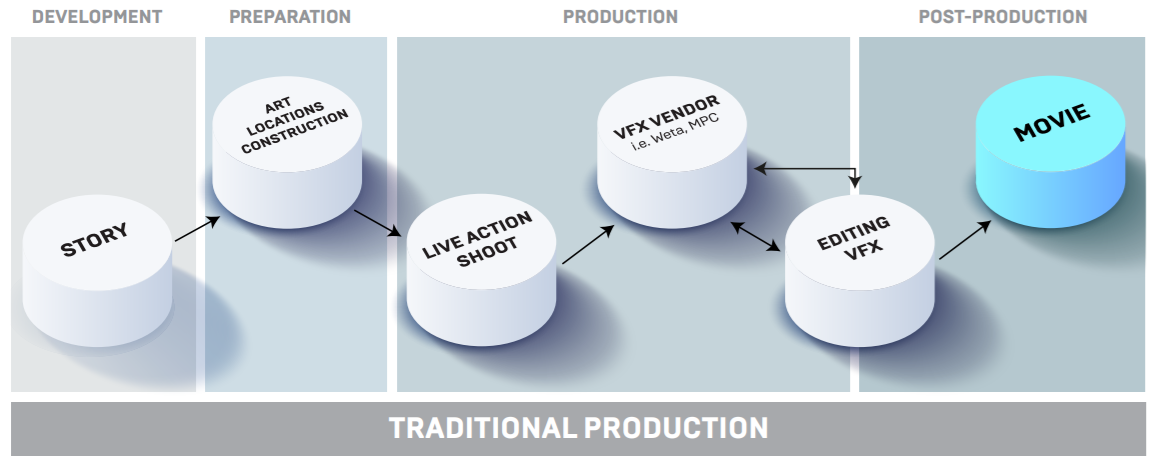
\includegraphics[width=15cm]{slika 2-1.png}
	\caption{Tradicionalna produkcija \cite{vpguide1}}
\end{figure}

\begin{figure}[htb]
	\centering
	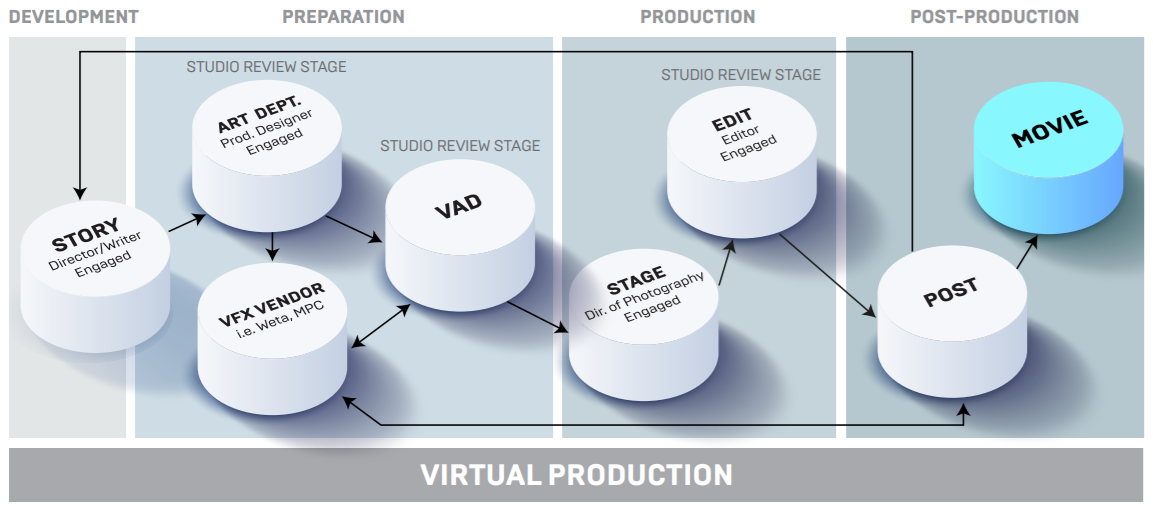
\includegraphics[width=15cm]{slika 2-2.png}
	\caption{Virtualna produkcija \cite{vpguide2}}
\end{figure}

\section{Slučajevi upotrebe}

\section{Opis prototipa}

\chapter{Upravljanje osvjetljenjem}

\section{DMX}

\subsection{Kontroleri}

\subsection{Rasvjetna tijela}

\subsection{Signalna komunikacija}

\section{Mrežni protokoli za prijenos podataka}

\subsection{Art-Net}

\subsection{sACN}

\chapter{Model rješenja}

\section{Simulacija osvjetljenja}

\section{Povezivanje sa prototipom}

\chapter{Zaključak}
Zaključak.

\raggedright
\bibliography{literatura}
\bibliographystyle{fer}

\begin{sazetak}
Sažetak na hrvatskom jeziku.

\kljucnerijeci{Ključne riječi, odvojene zarezima.}
\end{sazetak}

\engtitle{CONNECTING VIRTUAL AND REAL LIGHTING USING THE UNREAL SYSTEM}
\begin{abstract}
Abstract.

\keywords{Keywords.}
\end{abstract}

\end{document}
